\documentclass[11pt,psfig]{article}
\usepackage{epsfig}
\usepackage{times}
\usepackage{amssymb}
\usepackage{float}
\usepackage{listings}
\usepackage{graphicx}
\usepackage{caption}
\usepackage{subcaption}

\newcount\refno\refno=1
\def\ref{\the\refno \global\advance\refno by 1}
\def\ux{\underline{x}}
\def\uw{\underline{w}}
\def\bw{\underline{w}}
\def\ut{\underline{\theta}}
\def\umu{\underline{\mu}} 
\def\bmu{\underline{\mu}} 
\def\be{p_e^*}
\newcount\eqnumber\eqnumber=1
\def\eq{\the \eqnumber \global\advance\eqnumber by 1}
\def\eqs{\eq}
\def\eqn{\eqno(\eq)}

 \pagestyle{empty}
\def\baselinestretch{1.1}
\topmargin1in \headsep0.3in
\topmargin0in \oddsidemargin0in \textwidth6.5in \textheight8.5in
\begin{document}
\setlength{\parskip}{1.2ex plus0.3ex minus 0.3ex}


\thispagestyle{empty} \pagestyle{myheadings} \markright{Crater Lake Reconstruction}

\title{CS 217 Final Project: 3D Reconstruction of Crater Lake}
\author{Zachary DeStefano, 15247592}
\date{Due Date: June 11, 2015}

\maketitle

\vfill\eject

\newpage

\section{Background}

For this project, I attempted a 3D reconstruction of parts of Crater Lake National Park in Oregon.
\begin{figure}[H]
\centering
\includegraphics[width=\columnwidth]{craterLakeWinter.jpg}
\caption{Crater Lake during winter}
\end{figure}
Google Earth offers a 3D view of Crater Lake and my goal was something close to what it showed. There is an island in the middle of the lake called Wizard Island. I decided to focus on that island as well as nearby ridges for my reconstruction. \\
\\
I used pictures taken from different angles in order to do the reconstruction. In order to ensure that I had a wealth of pictures to use, I found high definition video and used a handful of the frames. That way I do not need to worry about using pictures that were taken at different times of the day or year.\\
\\
After looking at multiple high definition videos of Crater Lake, there were two scenes that I decided to attempt to reconstruct. The first one was taken from Merriam Point and it shows Wizard Island as well as nearby peaks. The second one was taken from different points on the surface of the lake and it shows two views of Wizard Island. The first scene had relatively little translational motion thus SFM did not work too well. The second scene had some translational motion thus SFM performed slightly better. 
\begin{figure}[H]
\centering
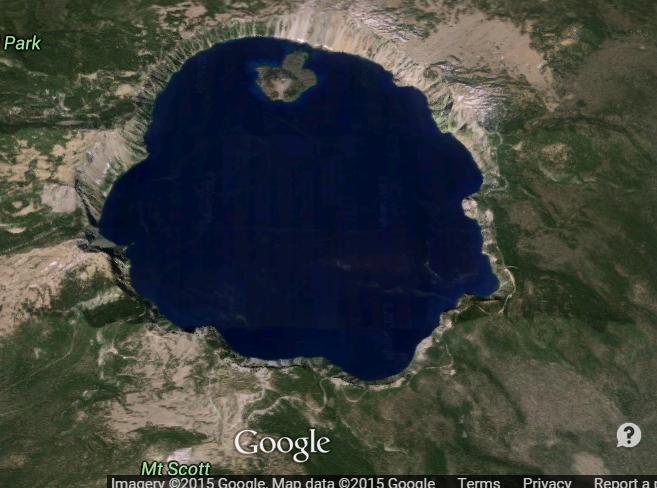
\includegraphics[width=\columnwidth]{googleEarthView1.png}
\caption{Top View of Crater Lake using Google Earth}
\end{figure}
\begin{figure}[H]
\centering
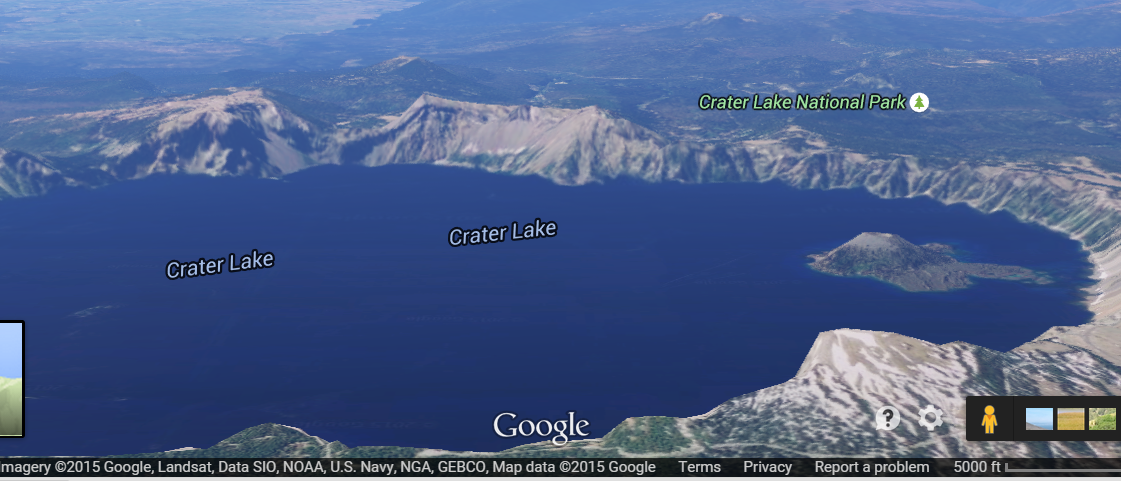
\includegraphics[width=\columnwidth]{googleEarthView2.png}
\caption{Side View of Crater Lake using Google Earth}
\end{figure}
\begin{figure}[H]
\centering
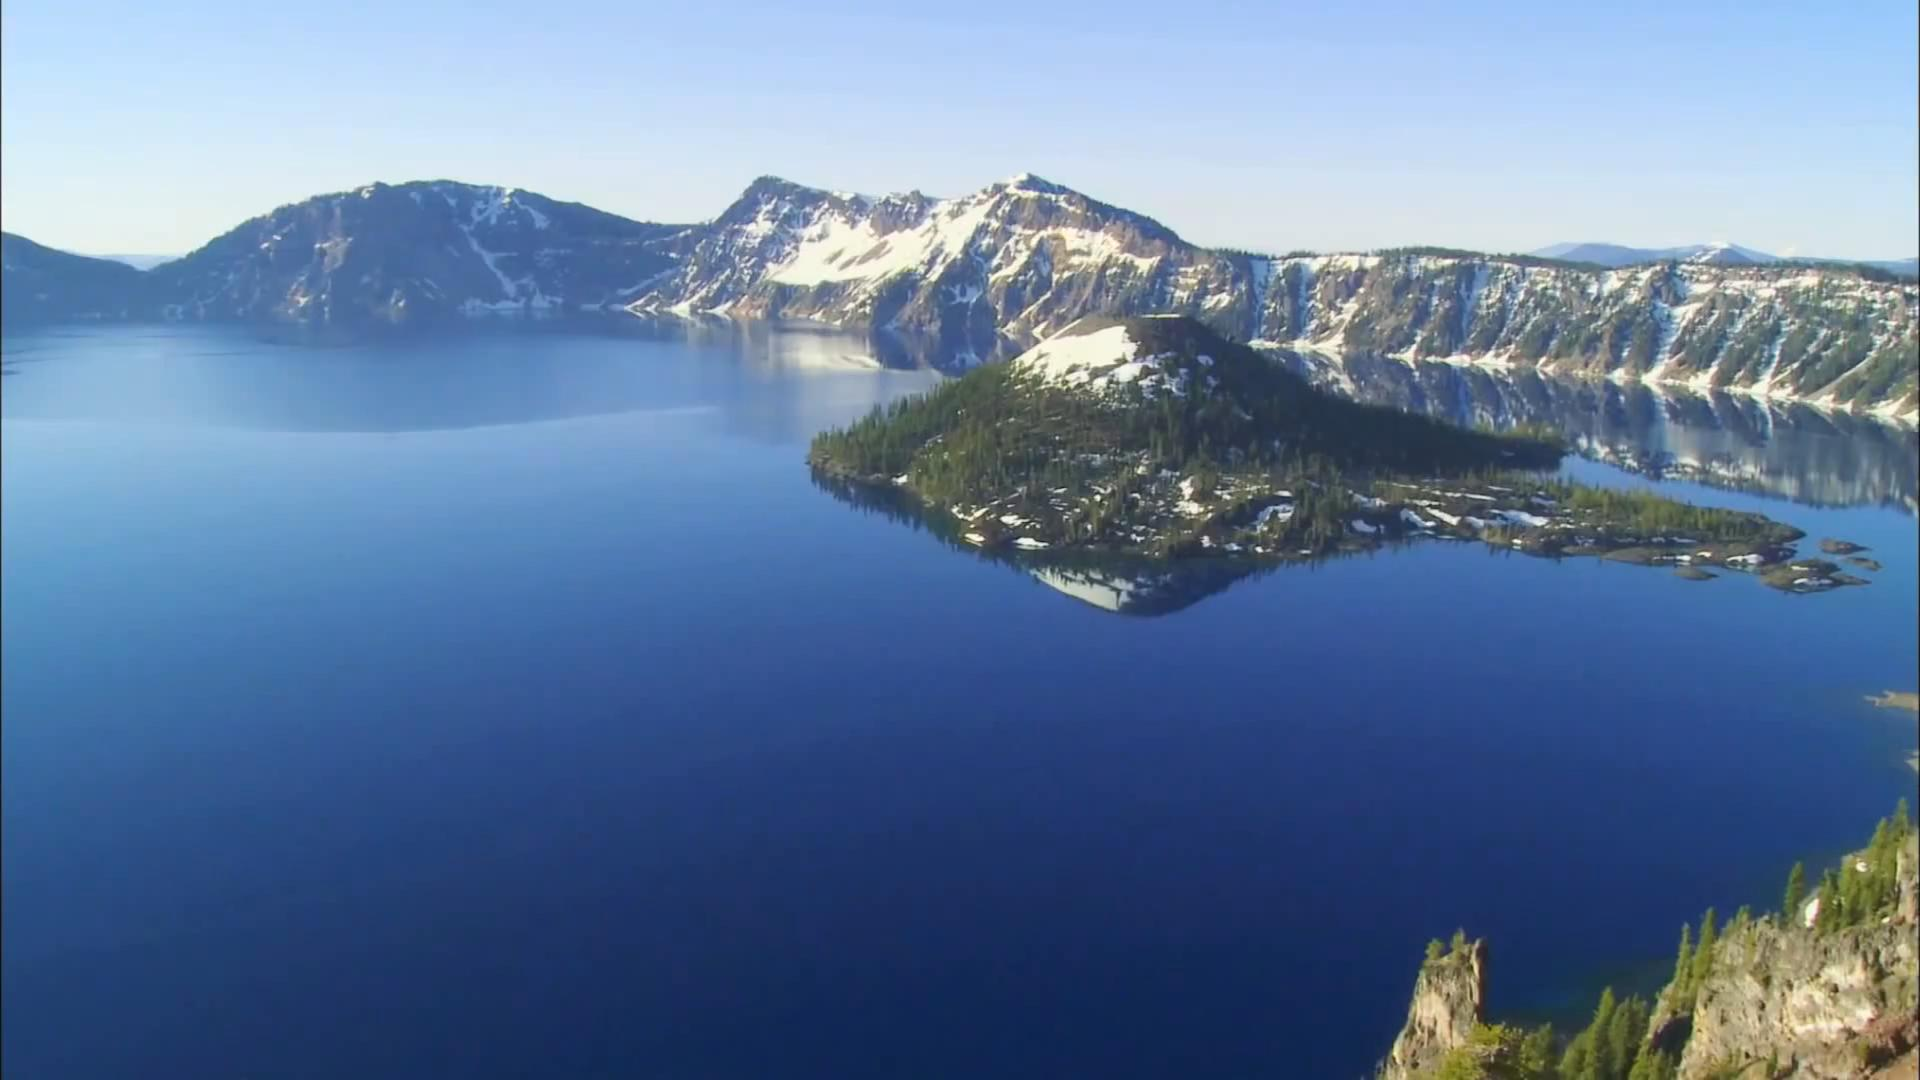
\includegraphics[width=\columnwidth]{sfmPics1J2/shot4.jpg}
\caption{Merriam Point Scene, Left Camera Shot}
\end{figure}
\begin{figure}[H]
\centering
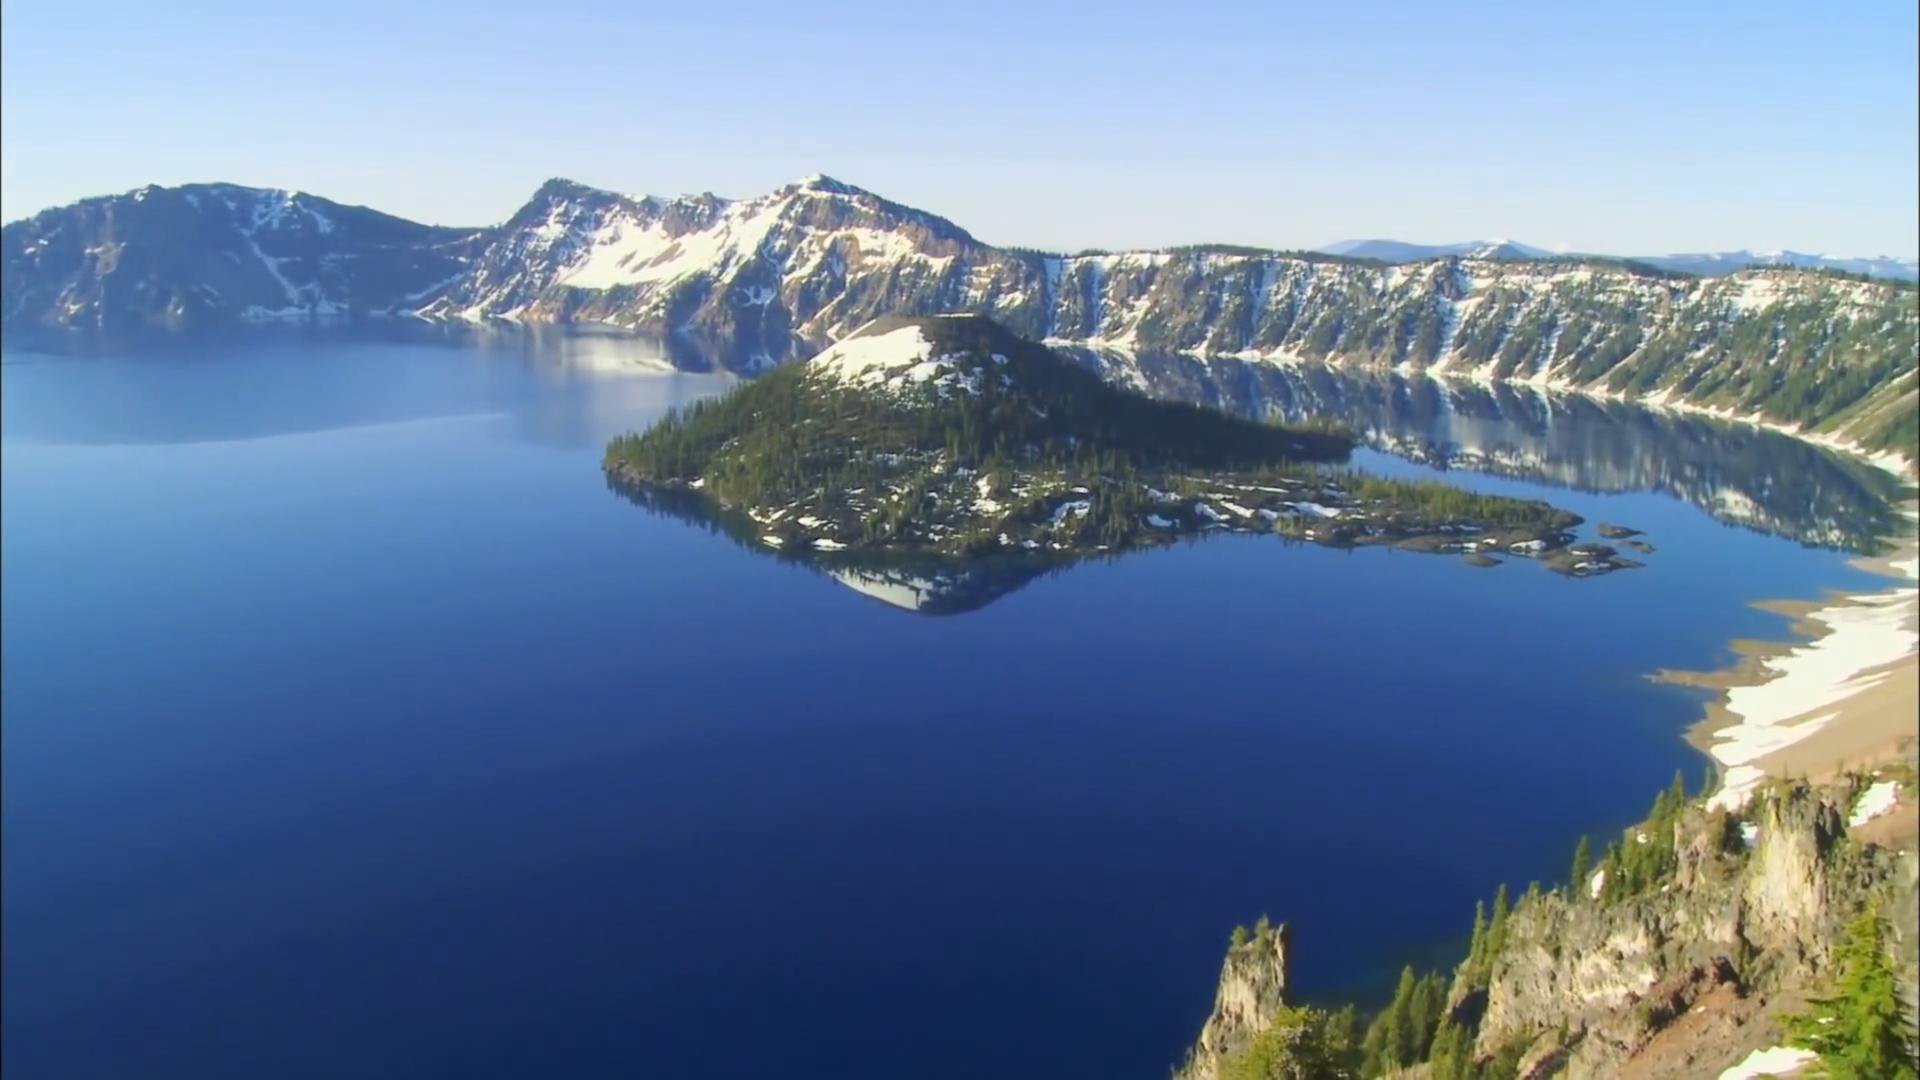
\includegraphics[width=\columnwidth]{sfmPics1J2/shot26.jpg}
\caption{Merriam Point Scene, Right Camera Shot}
\end{figure}
\begin{figure}[H]
\centering
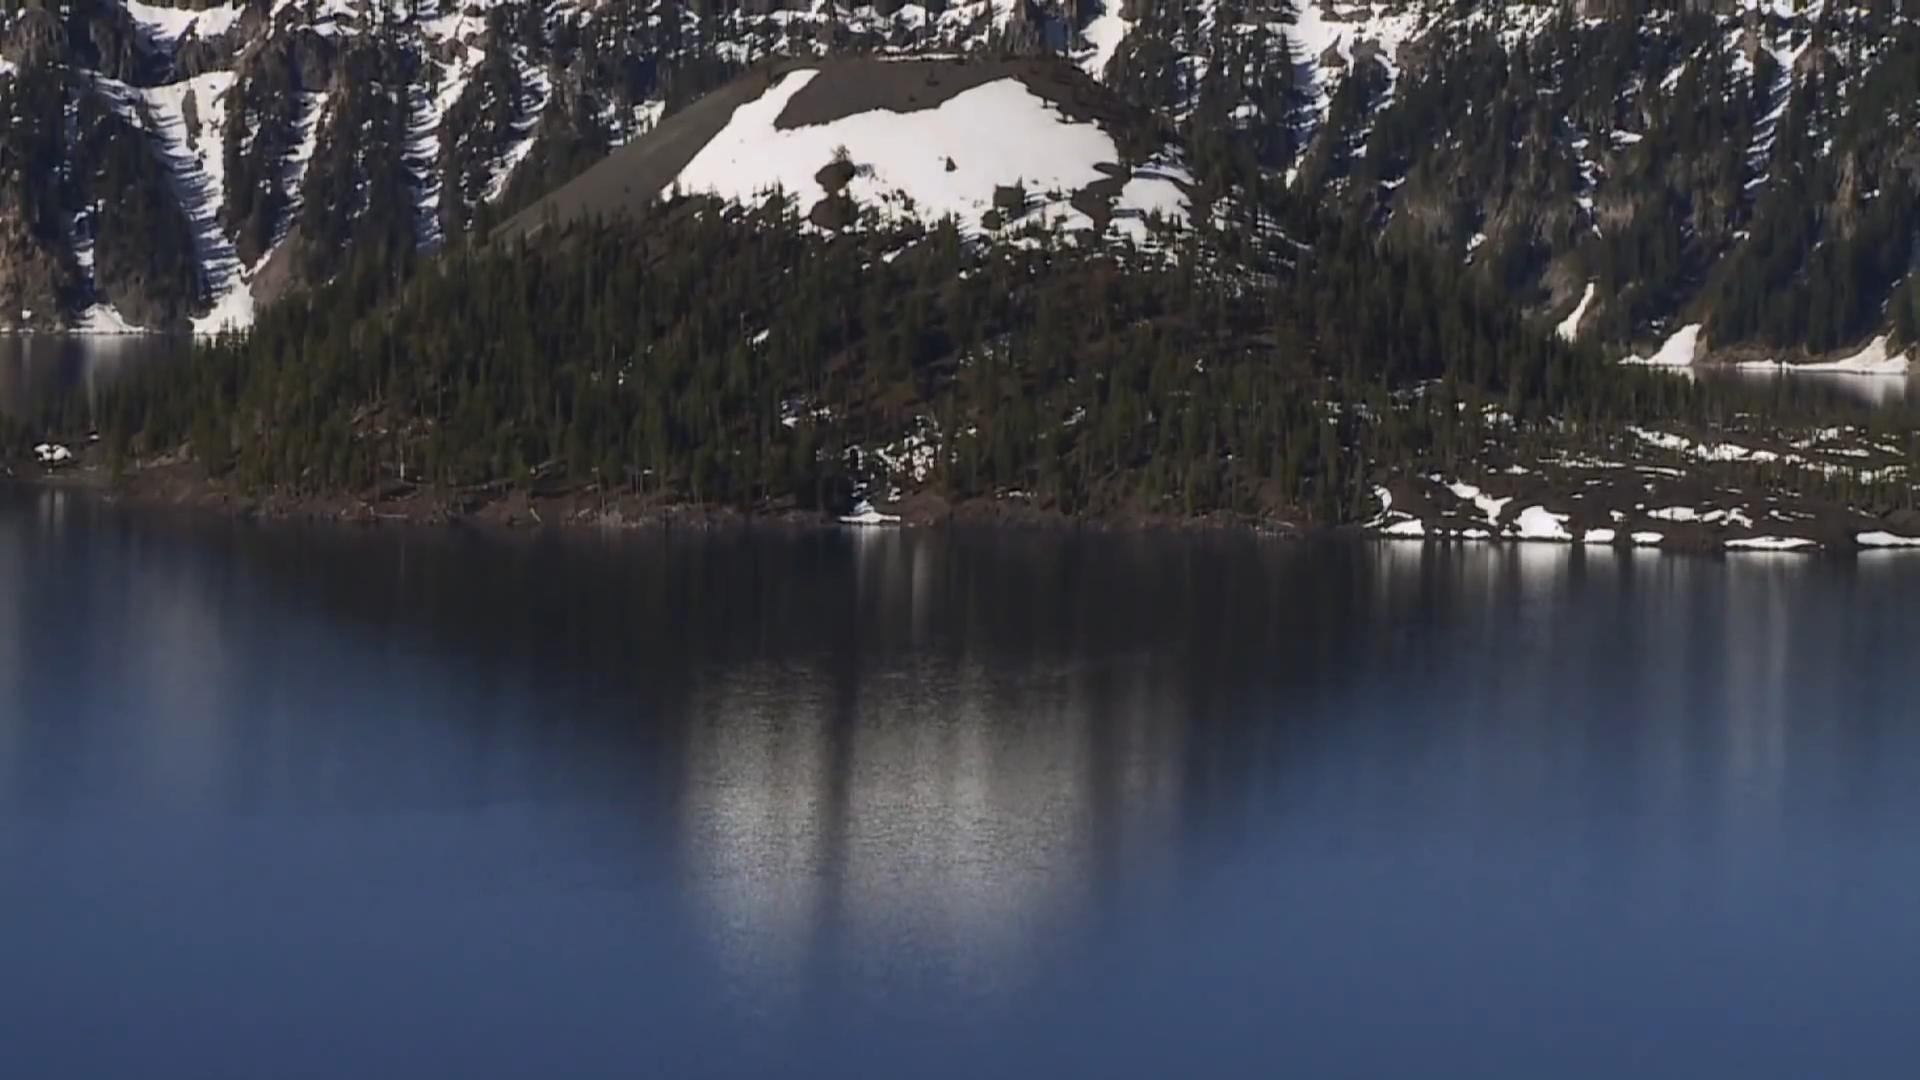
\includegraphics[width=\columnwidth]{sfmPics3/shot1.jpg}
\caption{Wizard Island Scene, close up shot}
\end{figure}
\begin{figure}[H]
\centering
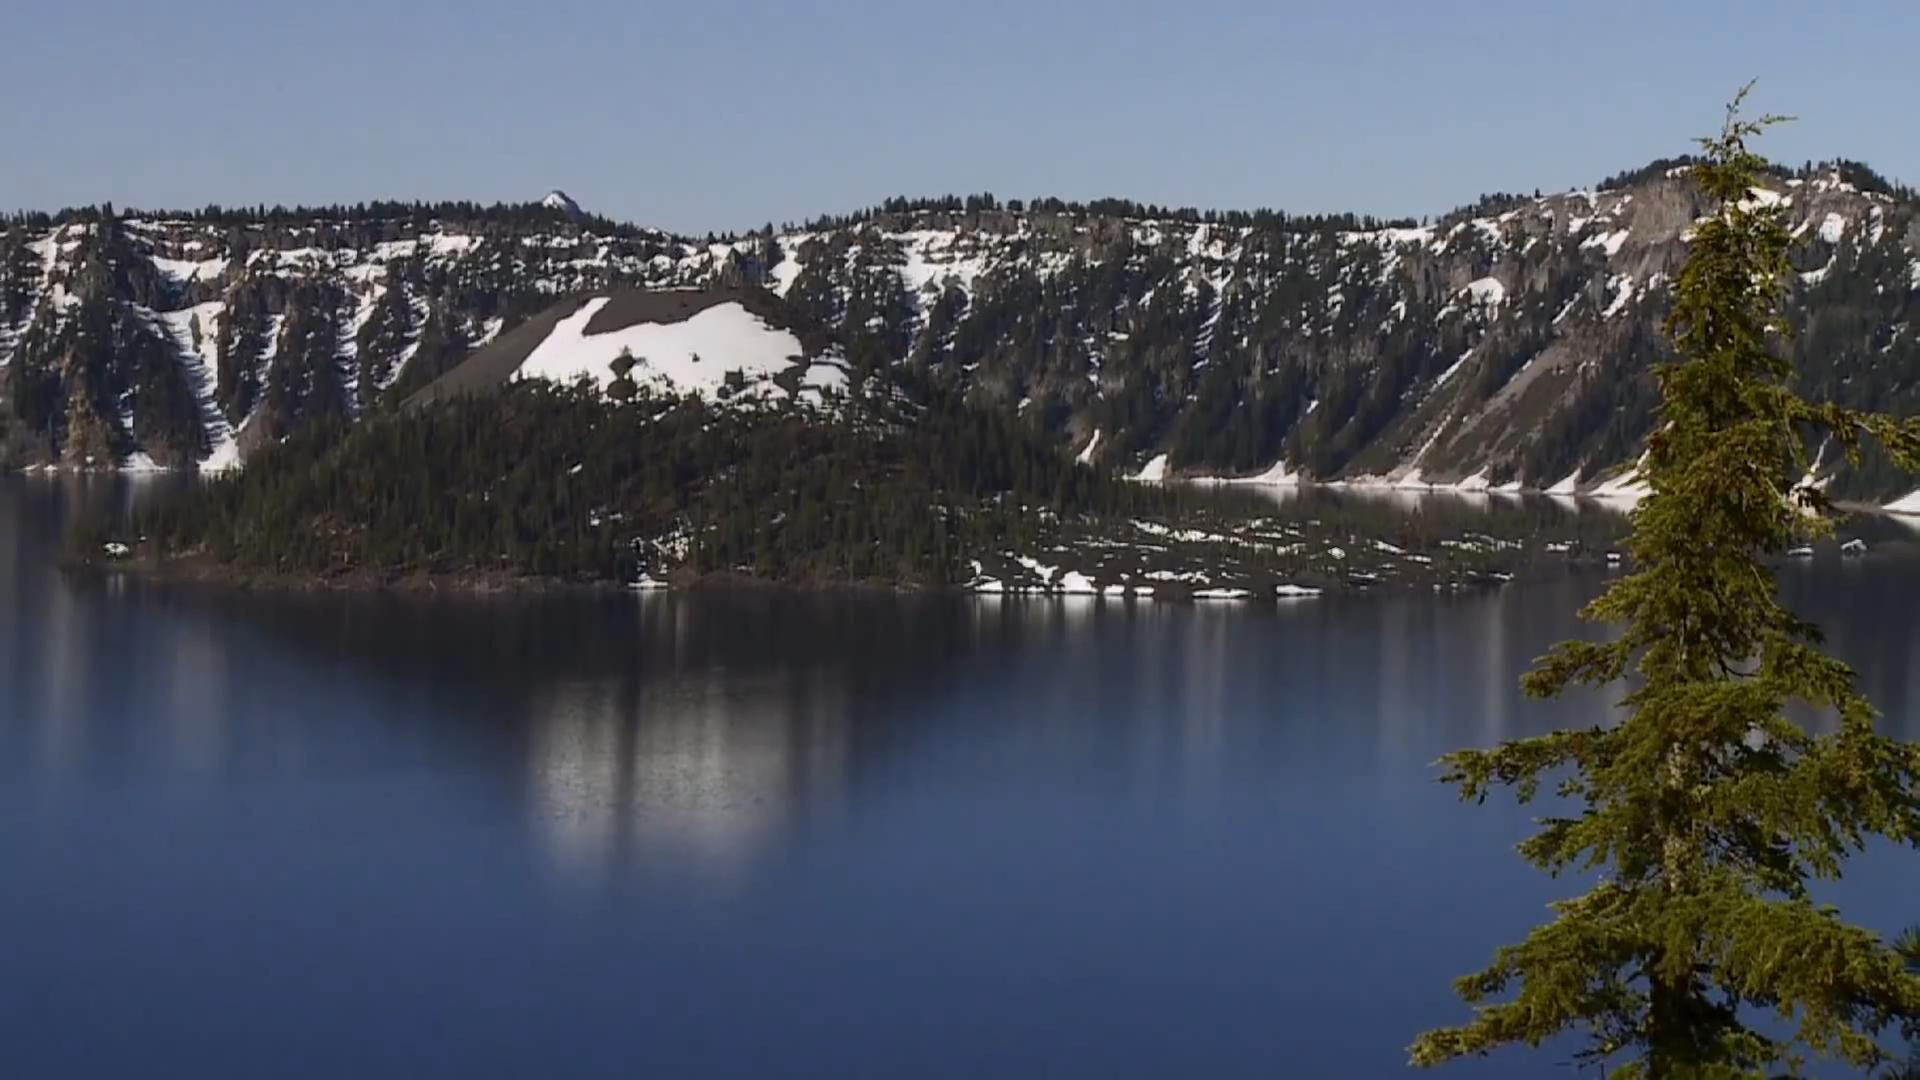
\includegraphics[width=\columnwidth]{sfmPics3/shot24.jpg}
\caption{Wizard Island Scene, further shot}
\end{figure}

\newpage

\section{Reconstruction of Merriam Point Scene}

The shots taken from Merriam Point had some distinguishable landmarks. There is existing spatial data on these landmarks thus I attempted to do calibration with the 3D data. 

\newpage

\section{Reconstruction of Wizard Island Scene}


%\begin{figure}[H]
%\centering
%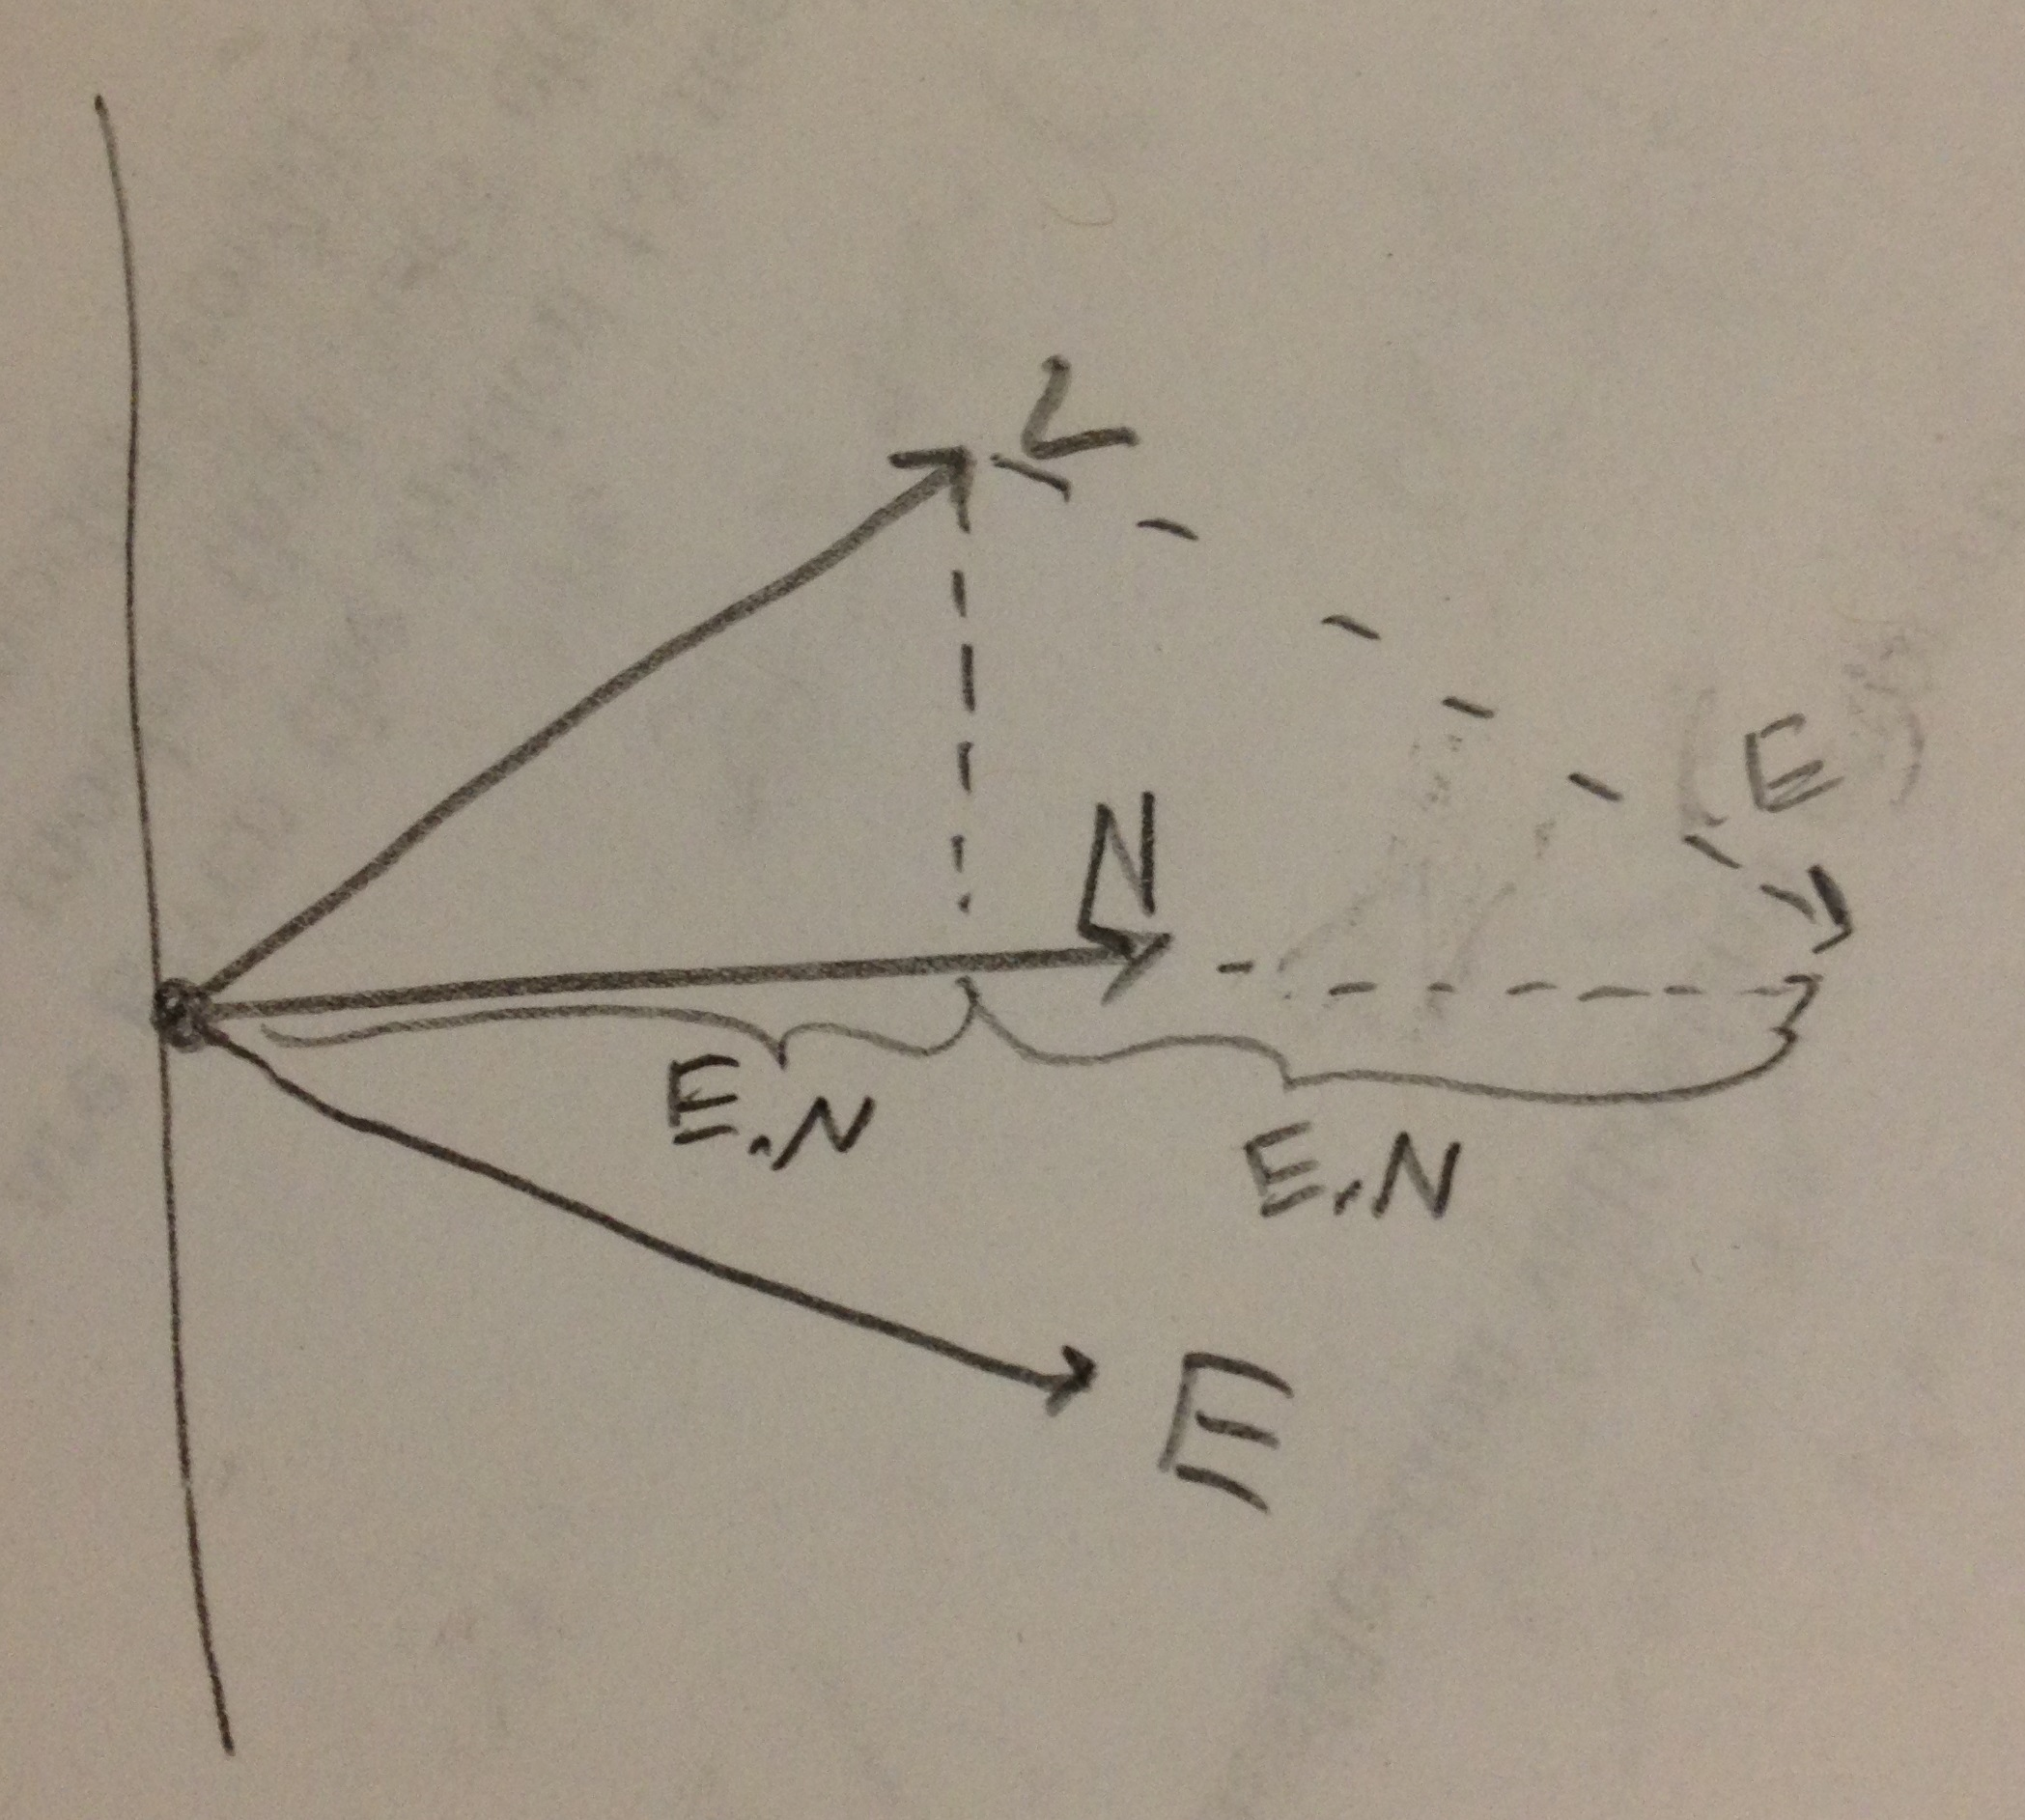
\includegraphics[height=3.5in]{prob1diagram.jpg}
%\caption{Illustration of normal vector N, light vector L, and viewing vector E and their relationships}
%\end{figure}




\end{document}








